\documentclass[12pt,a4paper]{article}
\usepackage[utf8]{inputenc}
\usepackage{amsmath}
\usepackage{amsfonts}
\usepackage{amssymb}
\usepackage{graphicx}
\usepackage[spanish]{varioref}
\usepackage{hyperref}
\usepackage{float}
\begin{document}
\setlength{\parindent}{0cm}

Titulo: Informe sobre aislaciones ópticas\\
version 0.2\\
18 de marzo de 2014\\
autor: Francisco Luis Zurita\\

\section{\textbf{Introducción}}

En este informe se presenta la aislación a usar en cada canal de entrada y salida de tensión digital previo y posterior al conversor DA del proyecto de adquisición de señales de un banco de motores.

\section{\textbf{Especificaciones}}

El aislador especificado a utilizar es el 6N137, un aislador óptico rápido de $10Mbit/s$, que satisface nuestros requerimientos ya que la señal digital mas rápida que se necesita aislar es de $52kHz$.

\section{\textbf{Diseño}}

El diseño del prototipo se enfoca en medir el comportamiento del aislador ante diferentes corrientes de excitación y condiciones de carga.
Dicho diseño se basa en la nota de aplicación 71\cite{AN}.\\

\begin{figure}[H]
\centering
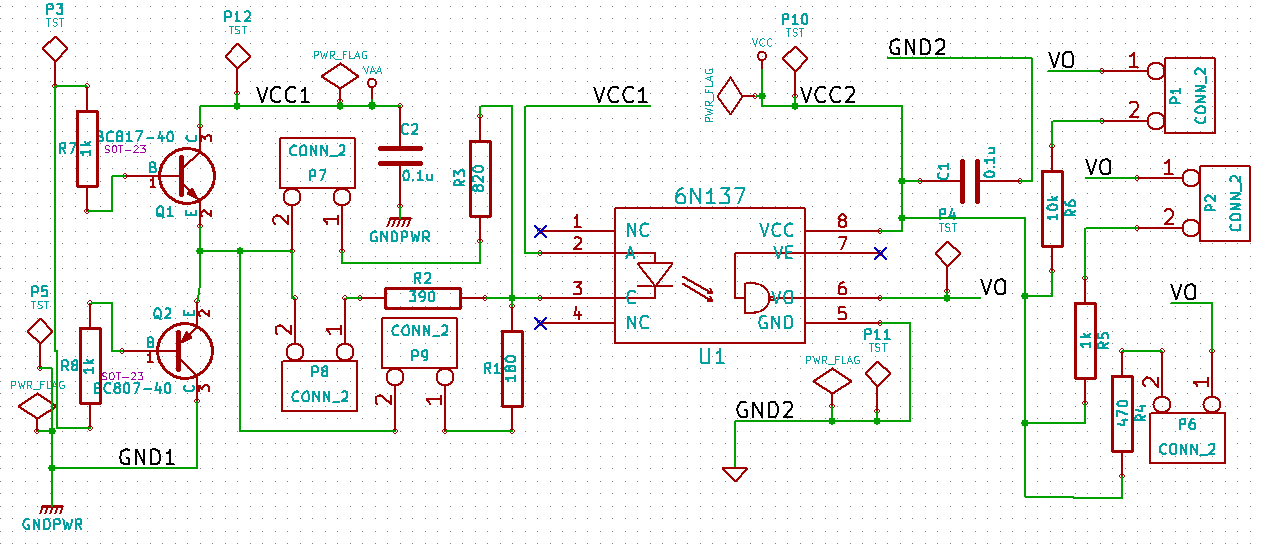
\includegraphics[scale=0.5]{img/optoaislacion.png}
\end{figure}


Para fijar la corriente de excitación se conmuta entre tres resistores por medio de un jumper. Las corrientes de entrada quedarán determinadas por el valor de dicha resistencia. Las mismas son:
$$
I_1=\frac{V_{CC1}-V_{LED}-V_{EC}}{R_1}=\frac{5V-1.4V-0.2V}{180\Omega}=18.9mA
$$
$$
I_2=\frac{V_{CC1}-V_{LED}-V_{EC}}{R_2}=\frac{5V-1.4V-0.2V}{390\Omega}=8.71mA
$$
$$
I_2=\frac{V_{CC1}-V_{LED}-V_{EC}}{R_3}=\frac{5V-1.4V-0.2V}
{820\Omega}=4.14mA
$$

El valor de $V_{LED}$ se obtiene de una curva de la hoja de datos y vale aproximadamente $1.4V$.\\
Para fijar la carga se conmuta entre tres resistores de pull-up por medio de un jumper. Esta resistencia junto con la de la punta del osciloscopio y la capacitancia de dicha punta conforman el circuito RC de carga a la salida.
Las cargas de salida son:
$$
(R_4||R_{osc})||C_{osc}=470\Omega ||10M\Omega || 10pF =470\Omega || 10pF
$$
$$
(R_5||R_{osc})||C_{osc}=1k\Omega ||10M\Omega || 10pF =999.9\Omega || 10pF
$$
$$
(R_6||R_{osc})||C_{osc}=10k\Omega ||10M\Omega || 10pF =9.99k\Omega || 10pF
$$

\newpage
\subsection{Listado de componentes}

\begin{tabular}{| l | l | l | l |}
\hline
Resistores & & &\\ \hline
Valor & Tolerancia & Cantidad & Referencia\\ \hline
180$\Omega$ & 5\% & 1 & $R_1$\\ \hline
390$\Omega$ & 5\% & 1 & $R_2$\\ \hline
820$\Omega$ & 5\% & 1 & $R_3$\\ \hline
470$\Omega$ & 5\% & 1 & $R_4$\\ \hline
1$k\Omega$ & 5\% & 3 & $R_{5,7,8}$\\ \hline
10$\Omega$ & 5\% & 1 & $R_6$\\ \hline
Capacitores & & & \\ \hline
Valor & Tolerancia & Cantidad & Referencia \\ \hline
0.1 $\mu F$ & 5\% & 2 & $C_{1,2}$  \\ \hline
Circuitos Integrados& & &\\ \hline
Modelo & Fabricante & Cantidad & Referencia \\ \hline
6N137 & ST & 1 & U1 \\ \hline
\end{tabular}

\newpage
\section{\textbf{Medición}}
\subsection{Banco de Medición}

Banco de Medición:

\begin{figure}[H]
\centering
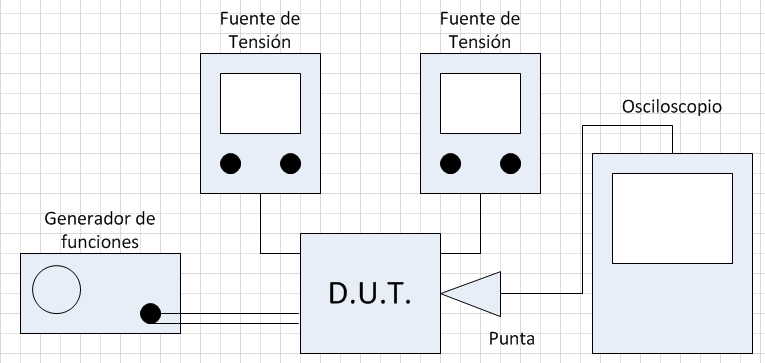
\includegraphics[width=\textwidth]{img/Banco.png}
\caption{Banco de medición}
\end{figure}

\begin{itemize}
\item Fuente de Tensión Fair FR-305A $0-30V$ 
\item Fuente de Tensión Zurich DF1730SB5A $0-30V$
\item Osciloscopio Fluke 192B 60MHz, 500MS/s\\
Sensibilidad 2mV - 100V/div\\
Rango de la base de tiempos: 10 ns - 2 min/div
\item Punta Fluke VP200 10:1 200MHz, 1.000 V CAT II/600 V CAT III (EN61010-1)
\item Generador de Funciones Hing Chang Sweep 9205\\
Frecuencia: $0.02Hz$ a $2MHz$ 7 rangos\\
Precisión: $\pm 5\%$ $(20KHz)$, $\pm 8\% (2MHz)$ 
\end{itemize}

Rise-time del conjunto generador-punta-osciloscopio: $56.8ns$.\\

Tensión de alimentación de entrada: $5V$\\
Tensión de alimentación de salida: $3.3V$\\
Señal de entrada: Tren de pulsos $0-5V$ a $10kHz$\\

\subsection{Imágenes}

<Reservado para foto>

\subsection{Resultados}

A continuación mostramos los resultados de las mediciones de retardo, rise-time (tiempo transcurrido entre el $10\%$ y el $90\%$ de la transición de estado bajo a estado alto de la señal) y fall-time (tiempo transcurrido entre el $10\%$ y el $90\%$ de la transición de estado alto a estado bajo de la señal).\\

\textbf{Rise-time}

\begin{figure}[H]
\centering
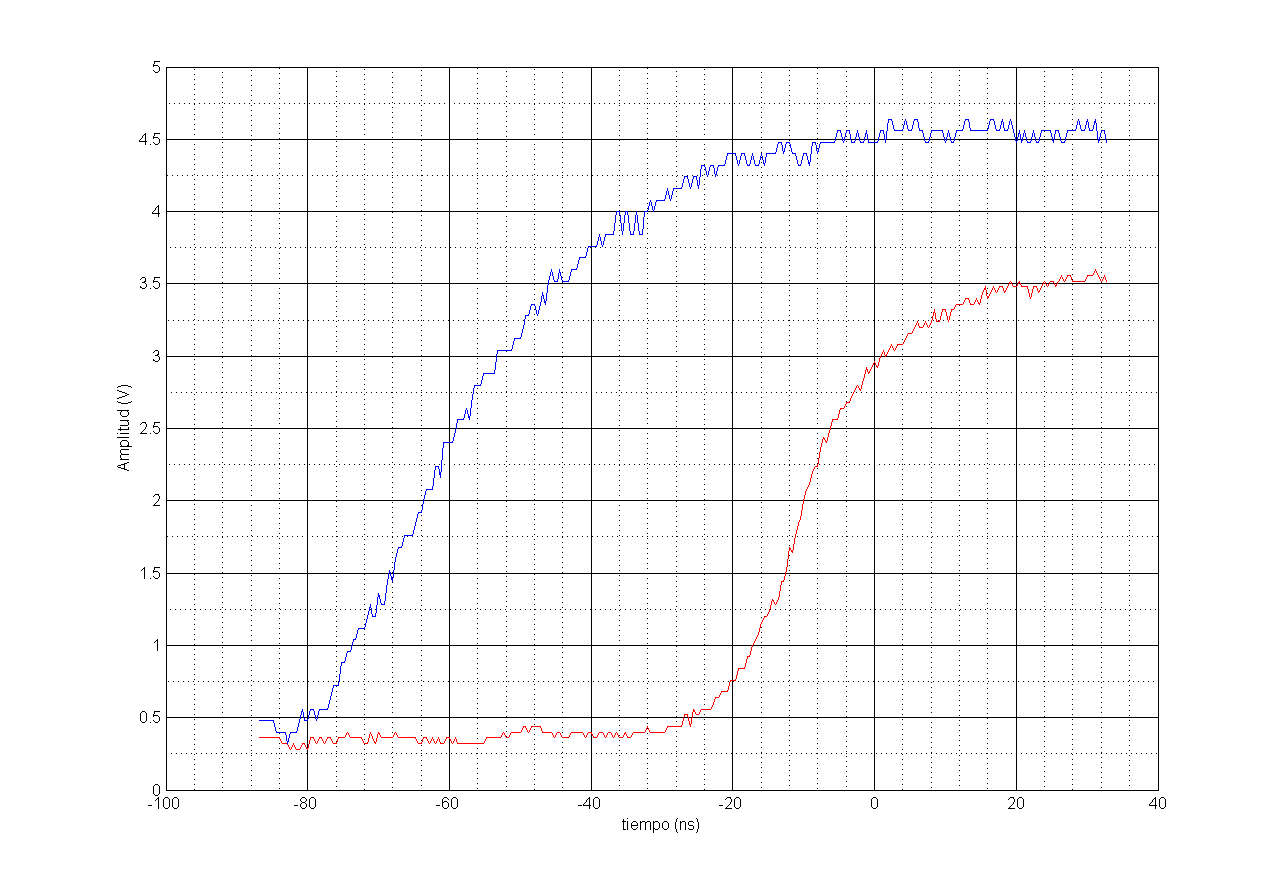
\includegraphics[width=\textwidth]{img/RT1.png}
\caption{Medición de rise-time usando $R_2=390\Omega$ y $R_4=470\Omega$: $39.6ns$}
\end{figure}

\begin{figure}[H]
\centering
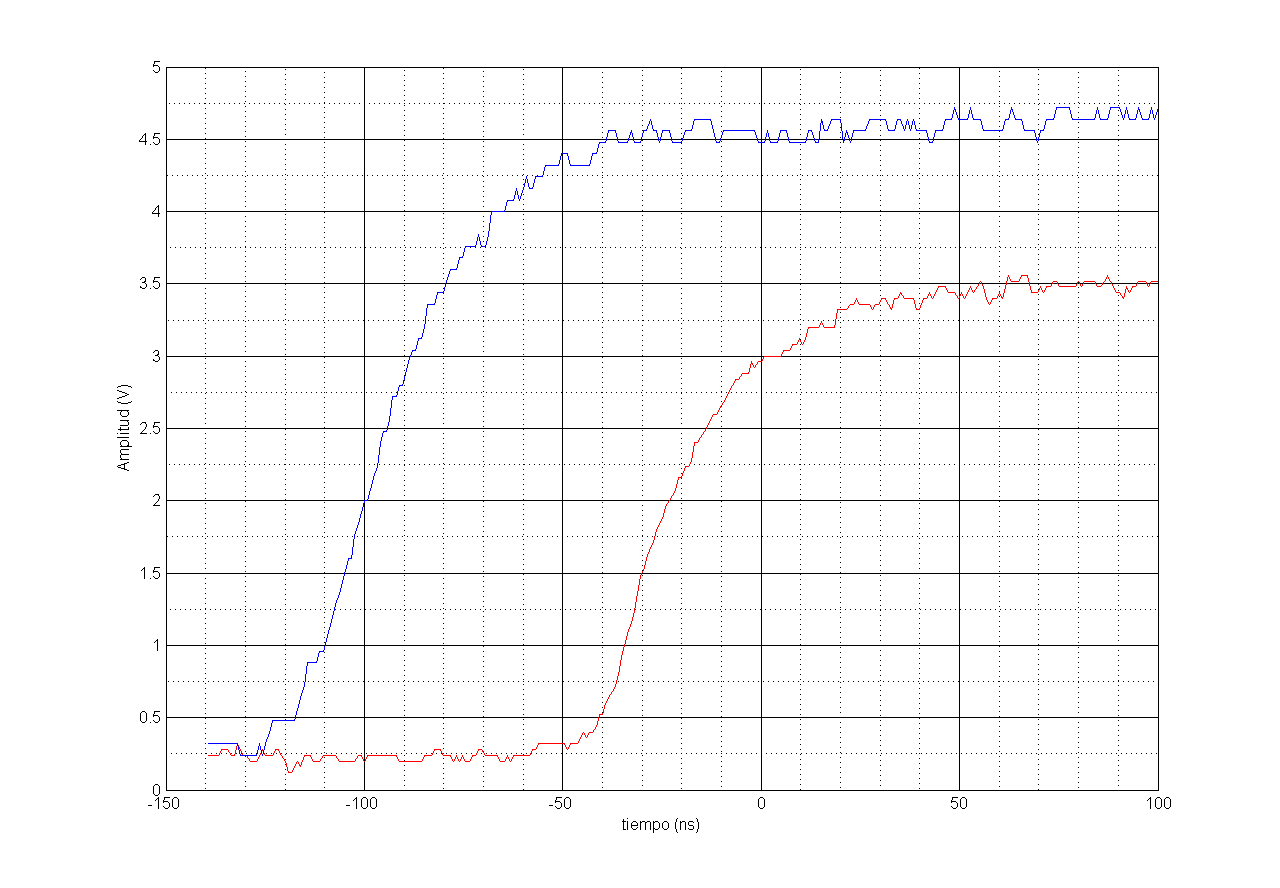
\includegraphics[width=\textwidth]{img/RT2.png}
\caption{Medición de rise-time usando $R_2=390\Omega$ y $R_4=1k\Omega$: $68.8ns$}
\end{figure}

\begin{figure}[H]
\centering
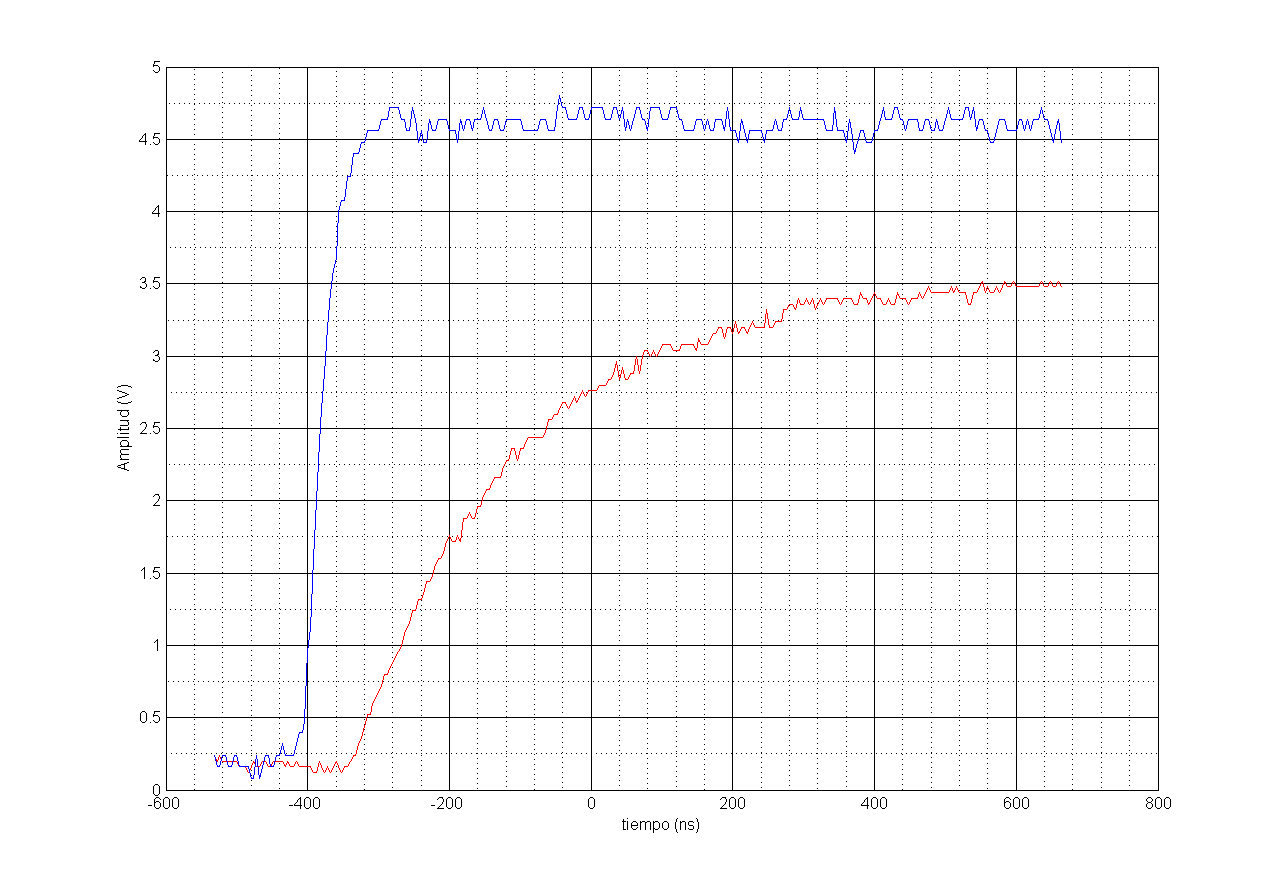
\includegraphics[width=\textwidth]{img/RT3.png}
\caption{Medición de rise-time usando $R_2=390\Omega$ y $R_4=10k\Omega$:
$628ns$}
\end{figure}

\begin{figure}[H]
\centering
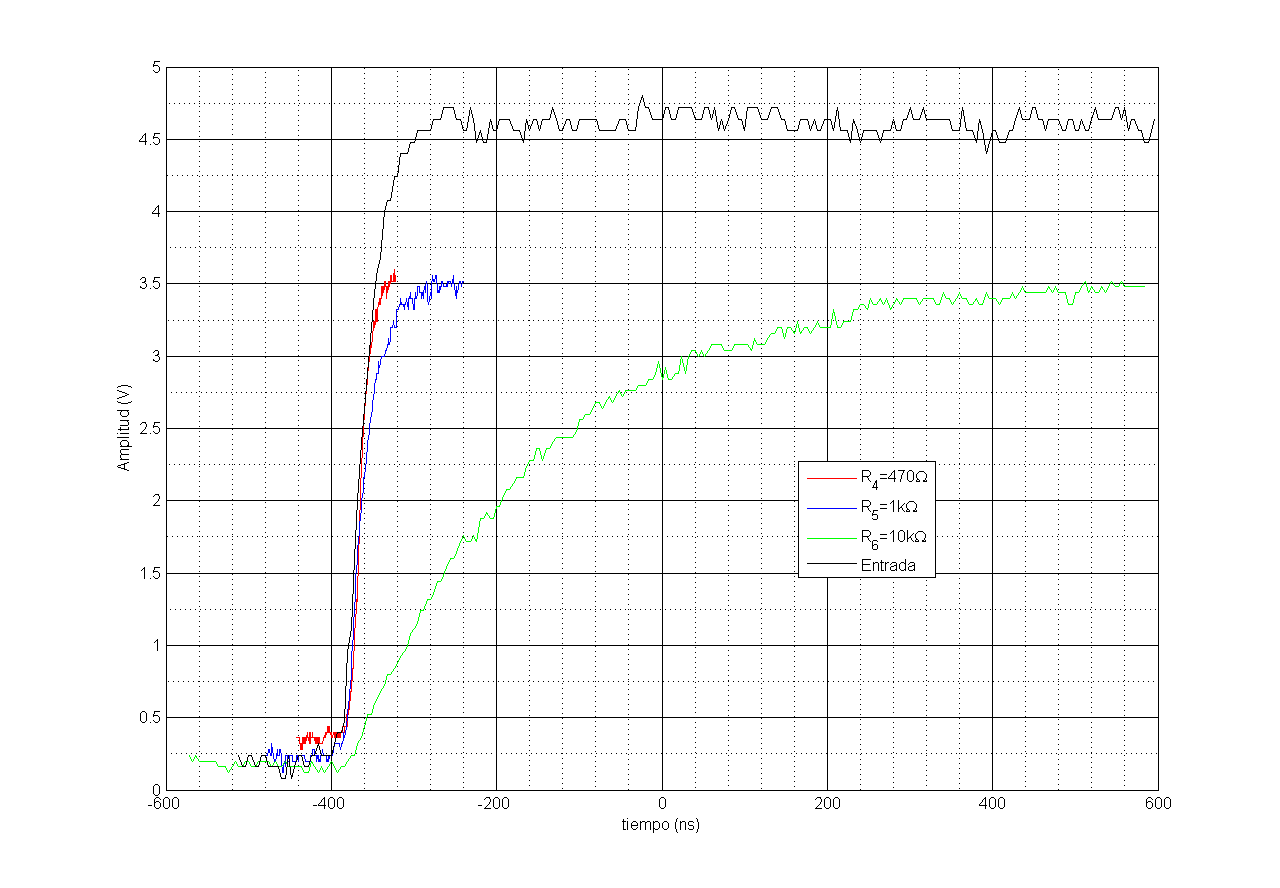
\includegraphics[width=\textwidth]{img/compRT.png}
\caption{Comparación de las figuras anteriores}
\end{figure}

\textbf{Fall-time}

\begin{figure}[H]
\centering
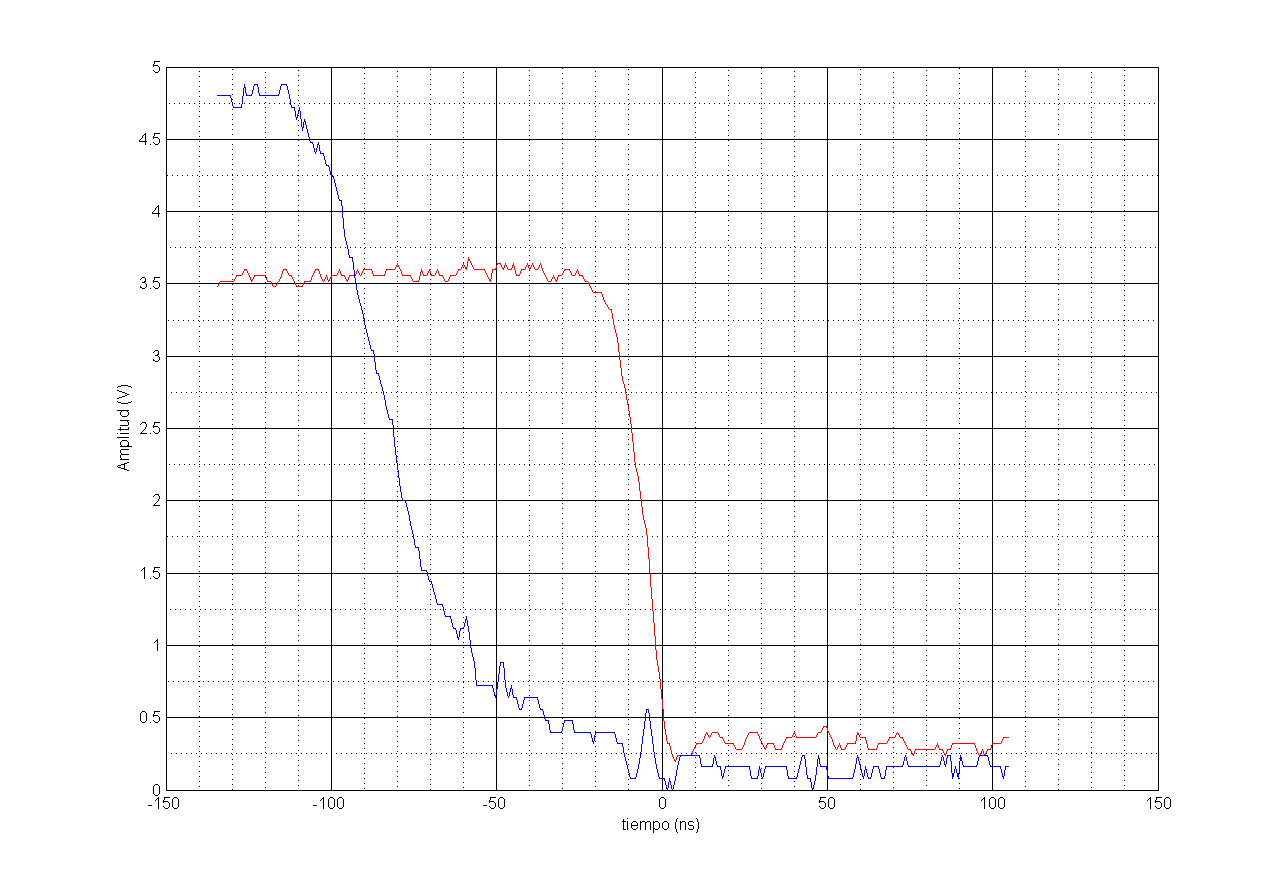
\includegraphics[width=\textwidth]{img/FT1.png}
\caption{Medición de fise-time usando $R_2=390\Omega$ y $R_4=470\Omega$: $12ns$}
\end{figure}

\begin{figure}[H]
\centering
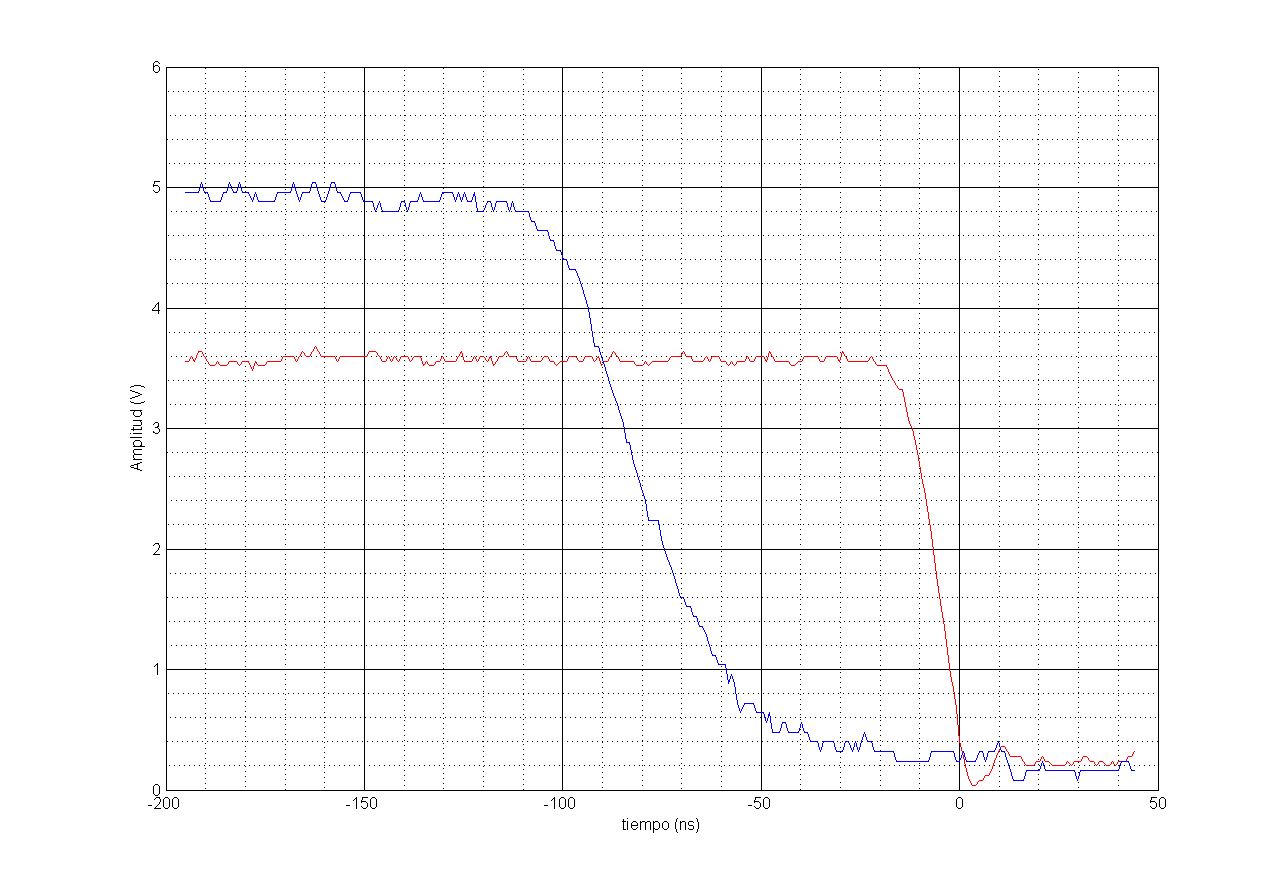
\includegraphics[width=\textwidth]{img/FT2.png}
\caption{Medición de fise-time usando $R_2=390\Omega$ y $R_4=1k\Omega$: $10ns$}
\end{figure}

\begin{figure}[H]
\centering
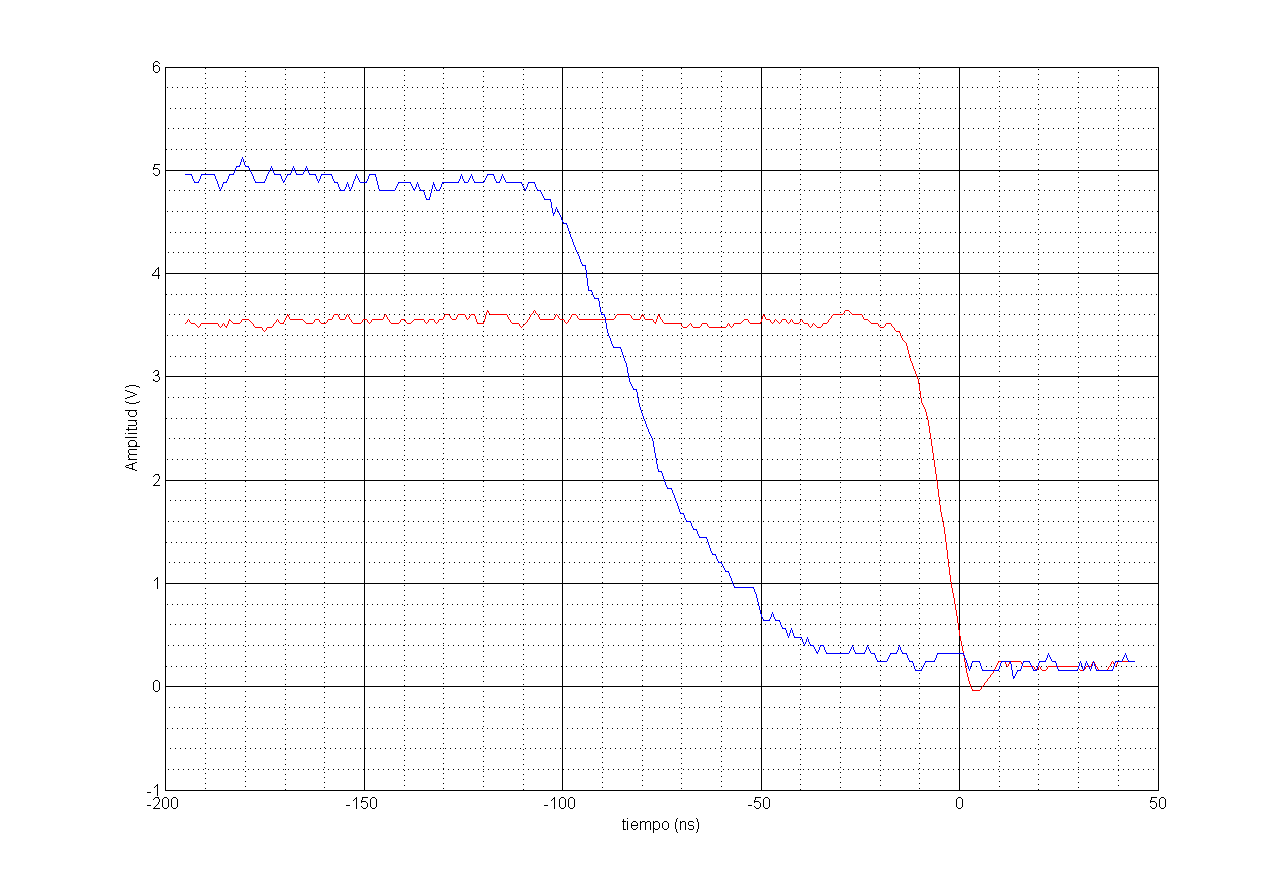
\includegraphics[width=\textwidth]{img/FT3.png}
\caption{Medición de fise-time usando $R_2=390\Omega$ y $R_4=10k\Omega$: $8.8ns$}
\end{figure}

\begin{figure}[H]
\centering
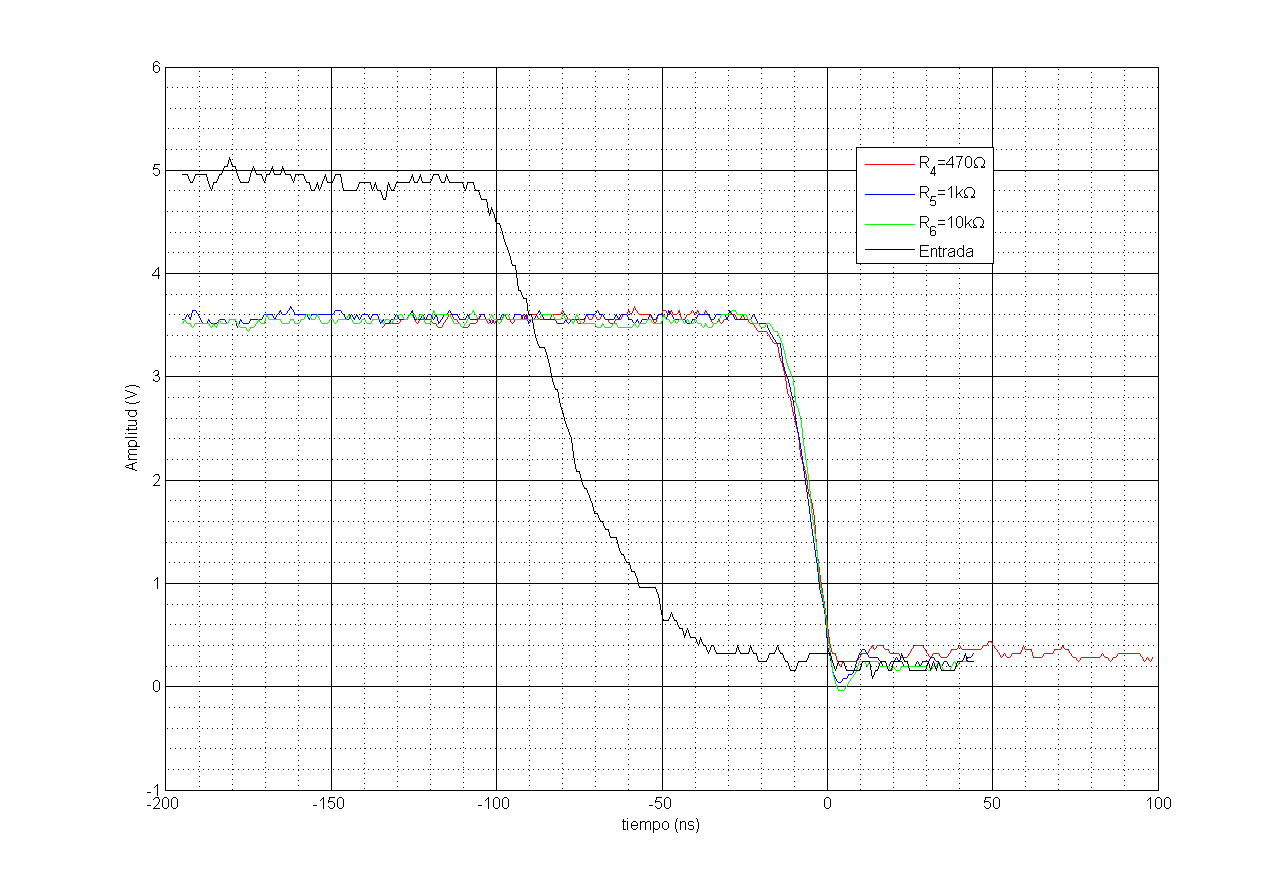
\includegraphics[width=\textwidth]{img/compFT.png}
\caption{Comparación de las figuras anteriores}
\end{figure}

\textbf{Retardo}

\begin{figure}[H]
\centering
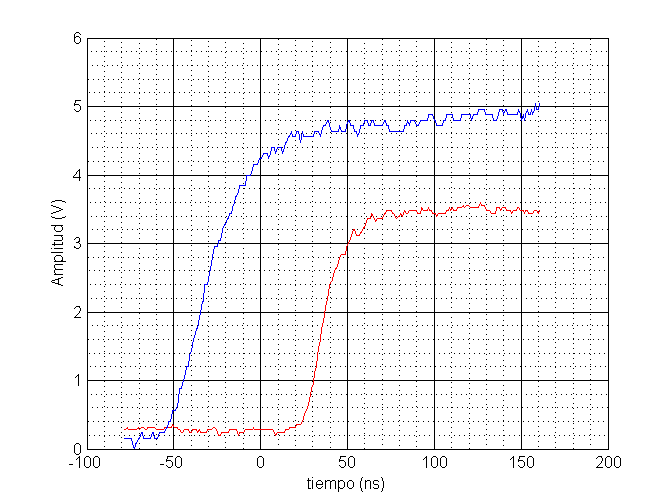
\includegraphics[width=\textwidth]{img/Delay1.png}
\caption{Medición de retardo usando $R_1=180\Omega$ y $R_5=1k\Omega$:$75ns$}
\end{figure}

\begin{figure}[H]
\centering
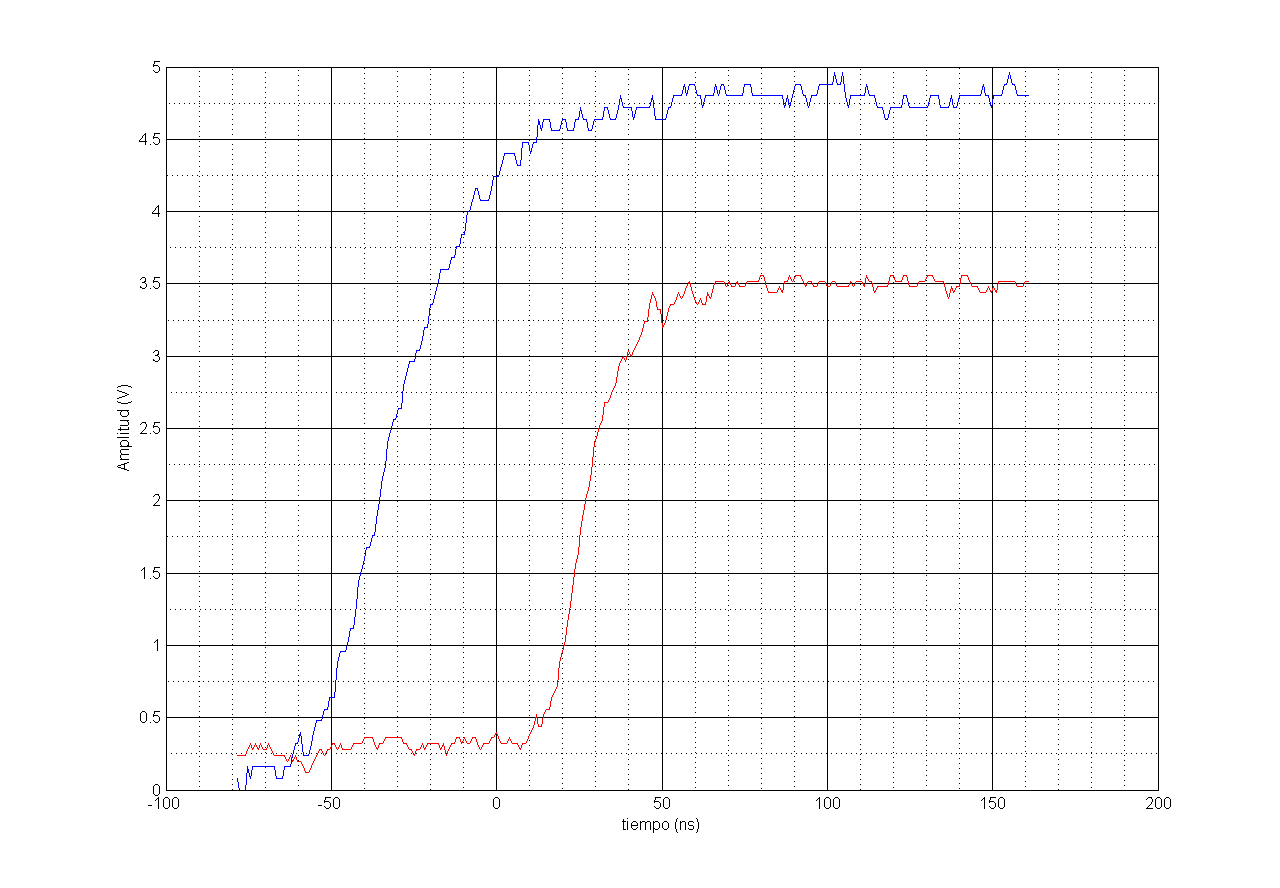
\includegraphics[width=\textwidth]{img/Delay2.png}
\caption{Medición de retardo usando $R_2=390\Omega$ y $R_5=1k\Omega$:$62.8ns$}
\end{figure}

\begin{figure}[H]
\centering
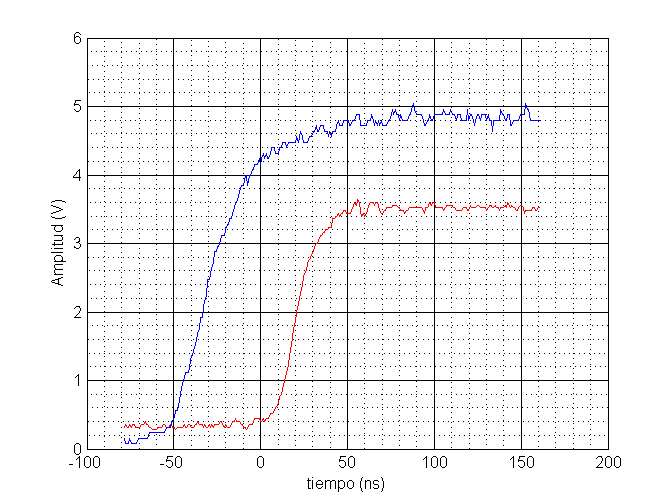
\includegraphics[width=\textwidth]{img/Delay3.png}
\caption{Medición de retardo usando $R_3=820\Omega$ y $R_5=1k\Omega$:$56ns$}
\end{figure}

\begin{figure}[H]
\centering
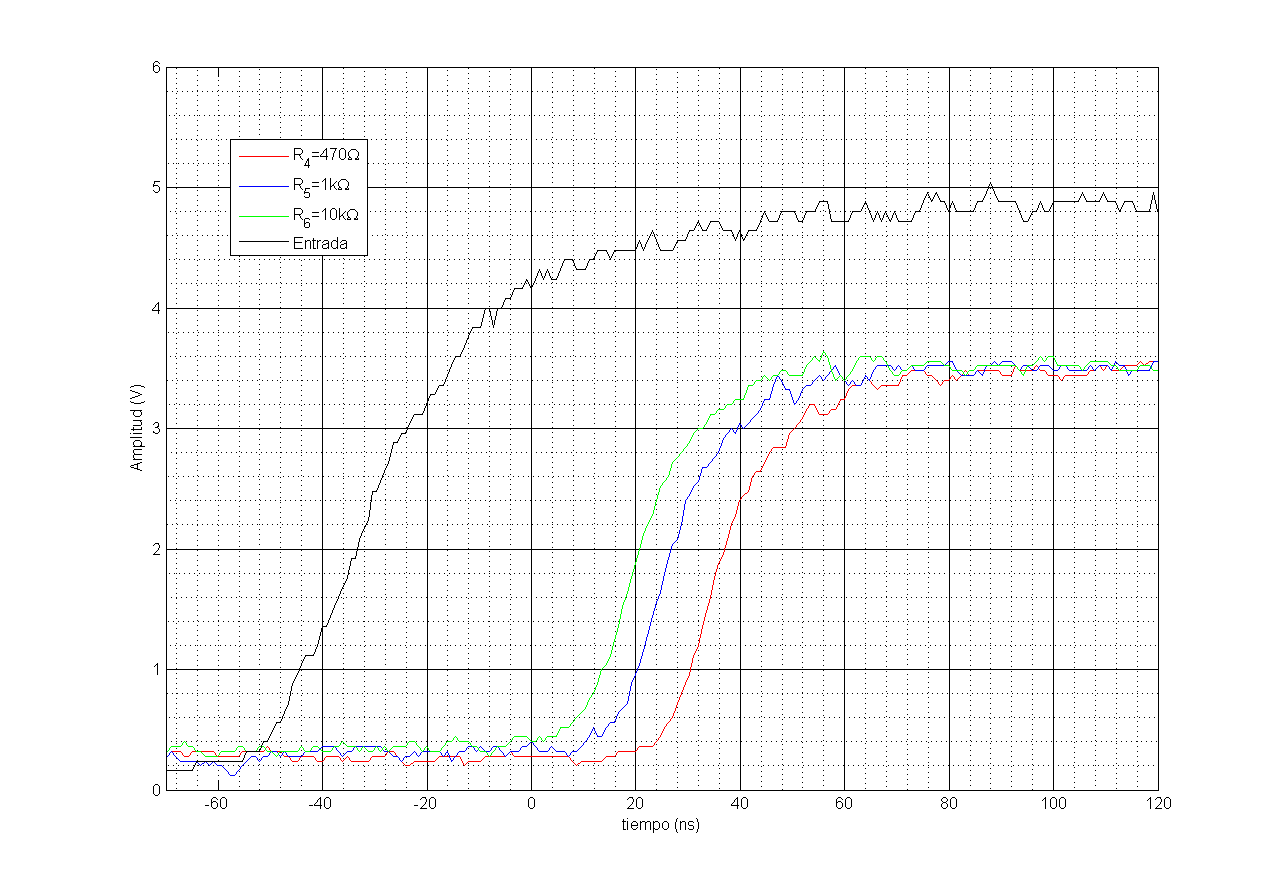
\includegraphics[width=\textwidth]{img/compDelay.png}
\caption{Comparación de las figuras anteriores}
\end{figure}

{\centering
\begin{tabular}{| c | c | c | c |} \hline
Corriente / Carga & $470\Omega$ & $1k\Omega$ & $10k\Omega$ \\ \hline
$I_1=18.9mA$ & $75ns$ & $75ns$ & $76ns$ \\ \hline 
$I_2=8.71mA$ & $62.8ns$ & $63.6ns$ & $62.8ns$ \\ \hline 
$I_3=4.14mA$ & $56ns$ & $55.2ns$ & $56.8ns$ \\ \hline 
\end{tabular}\\}
{\centering Tabla de valores de Retardo.\\}

{\centering
\begin{tabular}{| c | c | c | c |} \hline
Corriente / Carga & $470\Omega$ & $1k\Omega$ & $10k\Omega$ \\ \hline
$I_1=18.9mA$ & $32.8ns$ & $67.2ns$ & $624ns$ \\ \hline 
$I_2=8.71mA$ & $39.6ns$ & $68.8ns$ & $628ns$ \\ \hline 
$I_3=4.14mA$ & $32ns$ & $67.8ns$ & $620ns$ \\ \hline 
\end{tabular}\\}
{\centering Tabla de valores de rise-time.\\}

{\centering
\begin{tabular}{| c | c | c | c |} \hline
Corriente / Carga & $470\Omega$ & $1k\Omega$ & $10k\Omega$ \\ \hline
$I_1=18.9mA$ & $9.2ns$ & $8.8ns$ & $8.0ns$ \\ \hline 
$I_2=8.71mA$ & $12ns$ & $10ns$ & $8.8ns$ \\ \hline 
$I_3=4.14mA$ & $17.6ns$ & $16.8ns$ & $9.2ns$ \\ \hline 
\end{tabular}\\}
{\centering Tabla de valores de fall-time.\\}

Se observa de las mediciones anteriores que el retardo a la salida no depende de la condición de carga. A su vez, el rise-time y fall-time no dependen de la corriente de excitación.\\

\newpage
\begin{thebibliography}{1}
\bibitem{AN}\textit{AN71: 10MBd High-Speed Optocoupler Design Guide}, Noviembre 2011, Vishay Semiconductors.
\end{thebibliography}

\end{document}